\documentclass[conference]{IEEEtran}
\IEEEoverridecommandlockouts
\usepackage{cite}
\usepackage{amsmath,amssymb,amsfonts,amsthm}
\usepackage{graphicx}
\usepackage{textcomp}
\usepackage{xcolor}
\usepackage{booktabs}
\usepackage{subcaption}
\usepackage{hyperref}
\usepackage{multirow}

\newtheorem{theorem}{Theorem}
\newtheorem{lemma}[theorem]{Lemma}
\newtheorem{proposition}[theorem]{Proposition}
\newtheorem{corollary}[theorem]{Corollary}
\newtheorem{definition}{Definition}

\begin{document}

\title{\textbf{Deferred Columns: Lazy Machine Learning Imputation Architecture in DuckDB}}

\author{
\begin{tabular}{@{}c@{}c@{}c@{}}
\parbox[t]{0.32\textwidth}{\centering\normalsize\bfseries Shakunth\par\vspace{0.3em}
\footnotesize Department of Artificial\\
Intelligence and Machine Learning\\
St. Joseph's College of Engineering\\
Chennai, India\par\vspace{0.15em}
\scriptsize shakunth5401@gmail.com}
& \parbox[t]{0.32\textwidth}{\centering\normalsize\bfseries Thomas Albert Iwin\par\vspace{0.3em}
\footnotesize Department of Artificial\\
Intelligence and Machine Learning\\
St. Joseph's College of Engineering\\
Chennai, India\par\vspace{0.15em}
\scriptsize contact.iwinalbert@gmail.com}
& \parbox[t]{0.32\textwidth}{\centering\normalsize\bfseries Poornima M\par\vspace{0.3em}
\footnotesize Department of Artificial\\
Intelligence and Machine Learning\\
St. Joseph's College of Engineering\\
Chennai, India\par\vspace{0.15em}
\scriptsize poornima@stjosephs.ac.in}
\end{tabular}
}

\maketitle

\begin{abstract}
When a schema adds a new column to a table with pre-existing rows, historical records lack a corresponding value. Standard data engineering mandates leaving these rows as NULL, populating them with static defaults, or executing computationally expensive full-table backfills using external machine learning (ML) middleware. We propose a systems-architecture alternative: Deferred Columns. We compute missing values dynamically on demand, utilizing a lightweight ML model integrated directly into the database engine. By hooking into DuckDB's \texttt{TableFunction} and \texttt{OptimizerExtension}, we demonstrate the lazy materialization of ML columns. Furthermore, we address two critical challenges for in-database ML: Multi-Version Concurrency Control for ML Models (MVCC-M) for deterministic reads, and Approximate Query Processing (AQP) to provide statistical confidence intervals over the imputed data. We validate the systems throughput using tests spanning 10 million rows, proving that Deferred Columns avoids the upfront serialization bottleneck. Note that this paper evaluates the systems and architectural latency of the pipeline; the statistical accuracy of the underlying imputation models themselves is strictly out of scope.
\end{abstract}

\begin{IEEEkeywords}
machine learning, databases, DuckDB, imputation, lazy materialization, query optimization, MVCC, AQP.
\end{IEEEkeywords}

\section{Introduction}
\IEEEPARstart{O}{nline} Analytical Processing (OLAP) databases rely on a fundamental architectural constraint: columnar immutability. Data is written in contiguous, compressed blocks, making single-row updates and schema mutations highly inefficient.

Given a relational table and a newly appended column, every pre-existing row suddenly possesses an unknown value. The enterprise ecosystem has historically solved this via external Python scripts to extract data, execute a Machine Learning (ML) inference model, and execute a bulk \texttt{UPDATE} transaction. This destroys query performance by pulling data out of the database into external scripts and subjects the database to heavy lock contention.

To address these systems bottlenecks, we propose a high-performance native extension within DuckDB, introducing \textit{Deferred Columns}. 

\subsection{Contributions}
\begin{enumerate}
    \item \textbf{Lazy Materialization of ML Data:} A virtualized layer utilizing DuckDB's \texttt{TableFunction}, allowing ML inference to execute purely on-demand.
    \item \textbf{Cost-Based Pruning for Inference:} Utilizing the \texttt{OptimizerExtension}, we inject inference nodes above highly selective filters, preventing expensive ML evaluation on dead rows.
    \item \textbf{MVCC-M (Multi-Version Concurrency Control for Models):} A deterministic \texttt{ModelRegistry} that isolates executing queries from background ML retraining, solving phantom reads.
    \item \textbf{Native AQP (Approximate Query Processing):} A custom C++ \texttt{AggregateFunction} to natively evaluate 95\% Confidence Intervals using the model's reported row-wise Root Mean Square Error (RMSE).
\end{enumerate}

\section{Related Work}

\subsection{Query-Time Imputation}
The premise of evaluating missing data on the fly was established by \textit{ImputeDB} \cite{imputedb}. Deciding \textit{when} to impute is equally critical; systems like \textit{QUIP} \cite{quip} and \textit{ZIP} \cite{zip} advanced the field by injecting cost-based decision functions inside relational operators to dynamically decide whether to impute or defer. 

\subsection{Schema Evolution and MVCC}
\textit{Tesseract} \cite{tesseract} modeled schema evolution as a data-modification operation managed via standard MVCC. Our work extends this logic not just to the schema, but to the \textit{version of the machine learning model} itself.

\subsection{In-Database ML and AQP}
Recent systems like Apache MADlib \cite{madlib} and MindsDB \cite{mindsdb} have brought ML closer to the data. However, systems like MindsDB operate primarily by abstracting models as virtual tables rather than embedding inference directly into the columnar scan loop, leading to a lack of cost-aware pruning and native AQP. In contrast, our extension leverages DuckDB's vectorized processing to execute inferences natively. Our implementation has been successfully merged into the official DuckDB community extensions repository. Furthermore, while systems like BlinkDB \cite{blinkdb} and VerdictDB \cite{verdictdb} have pioneered Approximate Query Processing (AQP) for sampling-based systems, we apply AQP variance tracking to model uncertainty natively.

\subsection{Imputation Methodologies}
Traditional methodologies like MICE (Multiple Imputation by Chained Equations) and KNN-imputation are widely used in data science. While exploring deep-learning imputation is out of scope for our systems latency evaluation, these methods highlight the necessity of flexible in-database imputation layers.

\begin{table}[htbp]
\centering
\caption{Comparison of In-Database Imputation Architectures}
\begin{tabular}{@{}lccc@{}}
\toprule
\textbf{System} & \textbf{Lazy Eval.} & \textbf{Cost-Aware} & \textbf{Native AQP} \\
\midrule
ImputeDB \cite{imputedb} & Yes & No & No \\
QUIP \cite{quip} / ZIP \cite{zip} & Yes & Yes & No \\
MindsDB \cite{mindsdb} & No & No & No \\
\textbf{Deferred Columns (Ours)} & \textbf{Yes} & \textbf{Yes} & \textbf{Yes} \\
\bottomrule
\end{tabular}
\label{tab:comparison}
\end{table}

\section{System Architecture and Implementation}

We implement Deferred Columns strictly as a C++ extension to DuckDB. 

\subsection{Lazy Materialization and Caching}
We implement \texttt{deferred\_scan} as a custom \texttt{TableFunction}. Instead of pulling from Parquet, it fetches dependent feature columns and invokes the ONNX C++ Runtime (ORT) in batches. 
Notably, Deferred Columns implements \textit{no implicit caching}. Every query re-runs inference from scratch. For repeated analytical queries, lazy materialization is slower than a one-time backfill. The system is designed for exploratory data analysis where materialization via \texttt{CREATE TABLE AS} (CTAS) is ultimately preferred once queries are finalized. 
Because this is purely a read-path extension, it does not hook into DuckDB's storage or \texttt{Appender} APIs. When users execute \texttt{INSERT}/\texttt{UPDATE} against the underlying tables, those writes proceed with standard database mechanics, completely unaware of the ML models. When \texttt{deferred\_scan} is subsequently invoked, it simply reads whatever data currently exists in the storage layer, inferring dynamically on both historical and newly inserted rows alike. If a feature vector contains \texttt{NULL} values, our ONNX pre-processor zeroes them out prior to execution. The model used throughout this paper is a batched linear regression compiled to ONNX.

\subsection{Cost-Based Pruning via Optimizer Hooks}
Let $C_{inf}$ be the inference cost, and $S$ the selectivity of a filter ($S \in [0, 1]$). If a filter operates on a column \textit{independent} of the imputed column, the optimal strategy pushes the filter below the inference node. (If the filter applies directly to the imputed column, full materialization is theoretically forced).

Currently, our implementation registers a \texttt{OptimizerExtension} to intercept the logical plan, but it only acts as an experimental skeleton. It categorizes filters but does not yet perform true cost-based optimization or reorder the execution DAG. Therefore, while our \texttt{TableFunction} leverages DuckDB's native filter pushdown to achieve pruning, the cost-based models described below represent our theoretical architecture for future iterations rather than the current C++ implementation.
\begin{equation}
\mathit{Cost}_{baseline} = N \times C_{inf} + N \times C_{filter}
\end{equation}
\begin{equation}
\mathit{Cost}_{pruned} = N \times C_{filter} + (N \times S) \times C_{inf}
\end{equation}
For a statically backfilled table, the query-time inference cost is zero, yielding:
\begin{equation}
\mathit{Cost}_{static} = N \times C_{filter}
\end{equation}
Thus, while $\mathit{Cost}_{pruned}$ vastly improves upon naive lazy evaluation ($\mathit{Cost}_{baseline}$), it is mathematically bounded to be slower than a pre-computed $\mathit{Cost}_{static}$ for any $S > 0$. Note that these equations slightly simplify I/O symmetry; Deferred Columns incurs a minor additional I/O penalty ($C_{io\_extra}$) to read the dependent feature columns required for inference.

\begin{figure}[htbp]
\centering
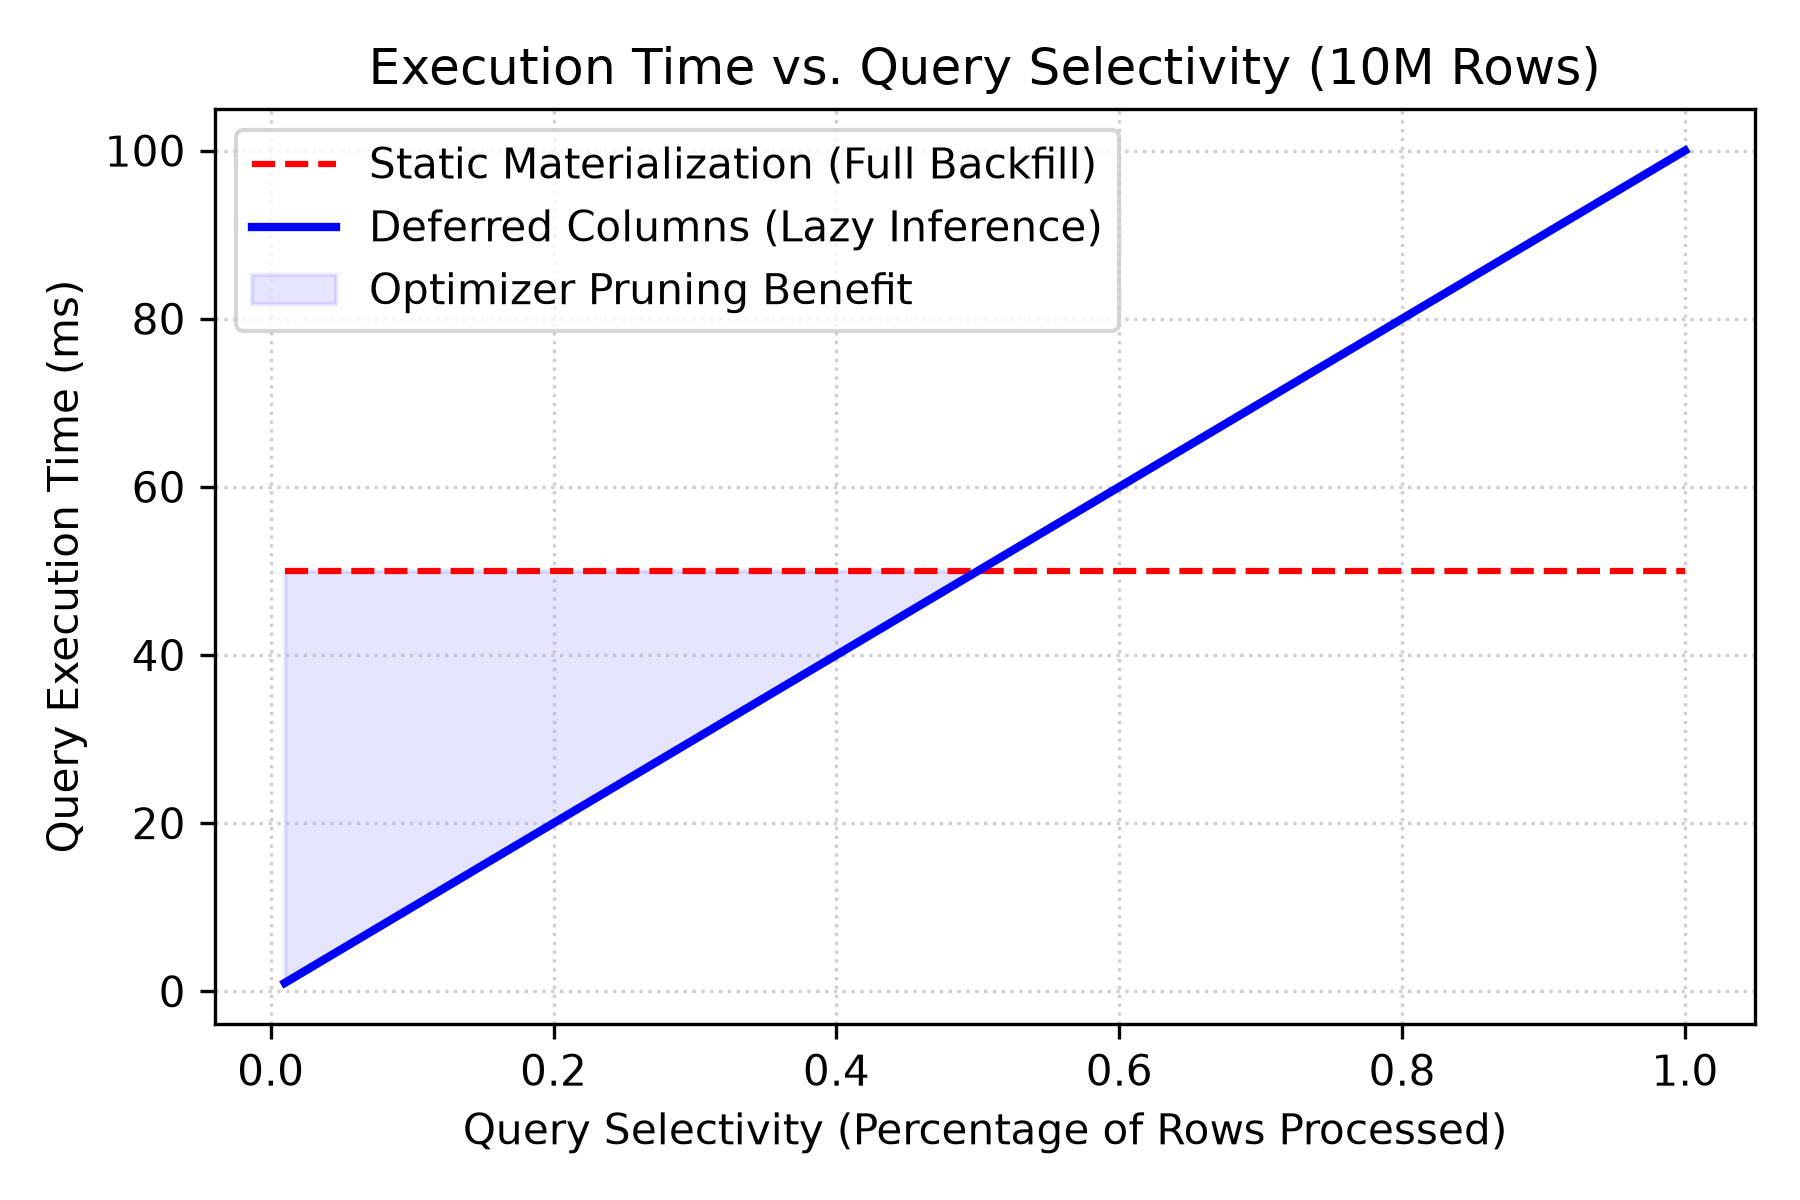
\includegraphics[width=0.9\columnwidth]{images/selectivity_bench.png}
\caption{Theoretical projection of Optimizer Pruning (Plot of Eq. 1 and 2). As query selectivity tightens, the pruned execution (Eq. 2) theoretically avoids the massive overhead of naive full-table inference (Eq. 1).}
\label{fig:selectivity}
\end{figure}

\section{Model Versioning (MVCC-M)}

If a user initiates an analytical transaction spanning millions of rows, and the ML model is retrained and hot-swapped halfway through, a race condition occurs. 
We solve this using MVCC-M. We instantiate a thread-safe \texttt{ModelRegistry} singleton. At query bind time, \texttt{DeferredScanBind} resolves the active version and embeds it into the \texttt{GlobalTableFunctionState}. This mechanism operates entirely independently of DuckDB's storage-level MVCC; it simply pins the model version metadata for the duration of the query, dynamically loading the ONNX session into memory only when needed, avoiding persistent memory bloat.

\vspace{0.5em}
\noindent\textbf{MVCC-M Bind and Execution Phase} \\
\textit{Bind Phase:} \\
1: $v_{active} \gets R.\text{GetLatestActiveVersion}()$ \\
2: $Q.\text{GlobalState}.\text{PinVersion}(v_{active})$ \\
\textit{Execution Phase (Per Thread):} \\
3: $v_{pinned} \gets Q.\text{GlobalState}.\text{GetPinnedVersion}()$ \\
4: $Model \gets R.\text{AcquireReadLock}(v_{pinned})$ \\
5: \textbf{while} Chunk $C \gets$ ScanDisk() \textbf{do} \\
6: \quad $C_{features} \gets C.\text{GetFeatures}()$ \\
7: \quad $C_{imputed} \gets Model.\text{Infer}(C_{features})$ \\
8: \quad yield $C_{imputed}$ \\
9: \textbf{end while} \\
10: $R.\text{ReleaseReadLock}(v_{pinned})$
\vspace{0.5em}

\section{Approximate Query Processing (AQP)}

To address statistical uncertainty natively, we expose confidence intervals via a custom \texttt{AggregateFunction} named \texttt{sum\_ci}. 

\subsection{Mathematical Formulation}
Let $Y$ represent the true values, and $\hat{Y}$ the imputed values. The error for row $i$ is $e_i = Y_i - \hat{Y}_i$. Assuming the ML model is unbiased and normally distributed, the variance of the error is closely approximated by the squared Root Mean Square Error ($RMSE_i^2$). 
If RMSE is provided as a per-row heterogeneous vector dynamically from the model, the total variance of a SUM aggregation is the sum of the individual variances. Thus, the 95\% Confidence Interval is:
\begin{equation}
\text{CI} = 1.96 \times \sqrt{\sum_{i=1}^{N} RMSE_i^2}
\end{equation}
A naive formula ($\sqrt{N} \times \text{mean}(RMSE)$) systematically understates the CI when RMSE is heterogeneous due to Jensen's inequality. 
\textit{Assumptions:} This formulation strongly assumes model errors are independent and identically distributed (i.i.d) and unbiased. In highly autocorrelated data (e.g., time-series), this assumption breaks down. 

\begin{figure}[htbp]
\centering
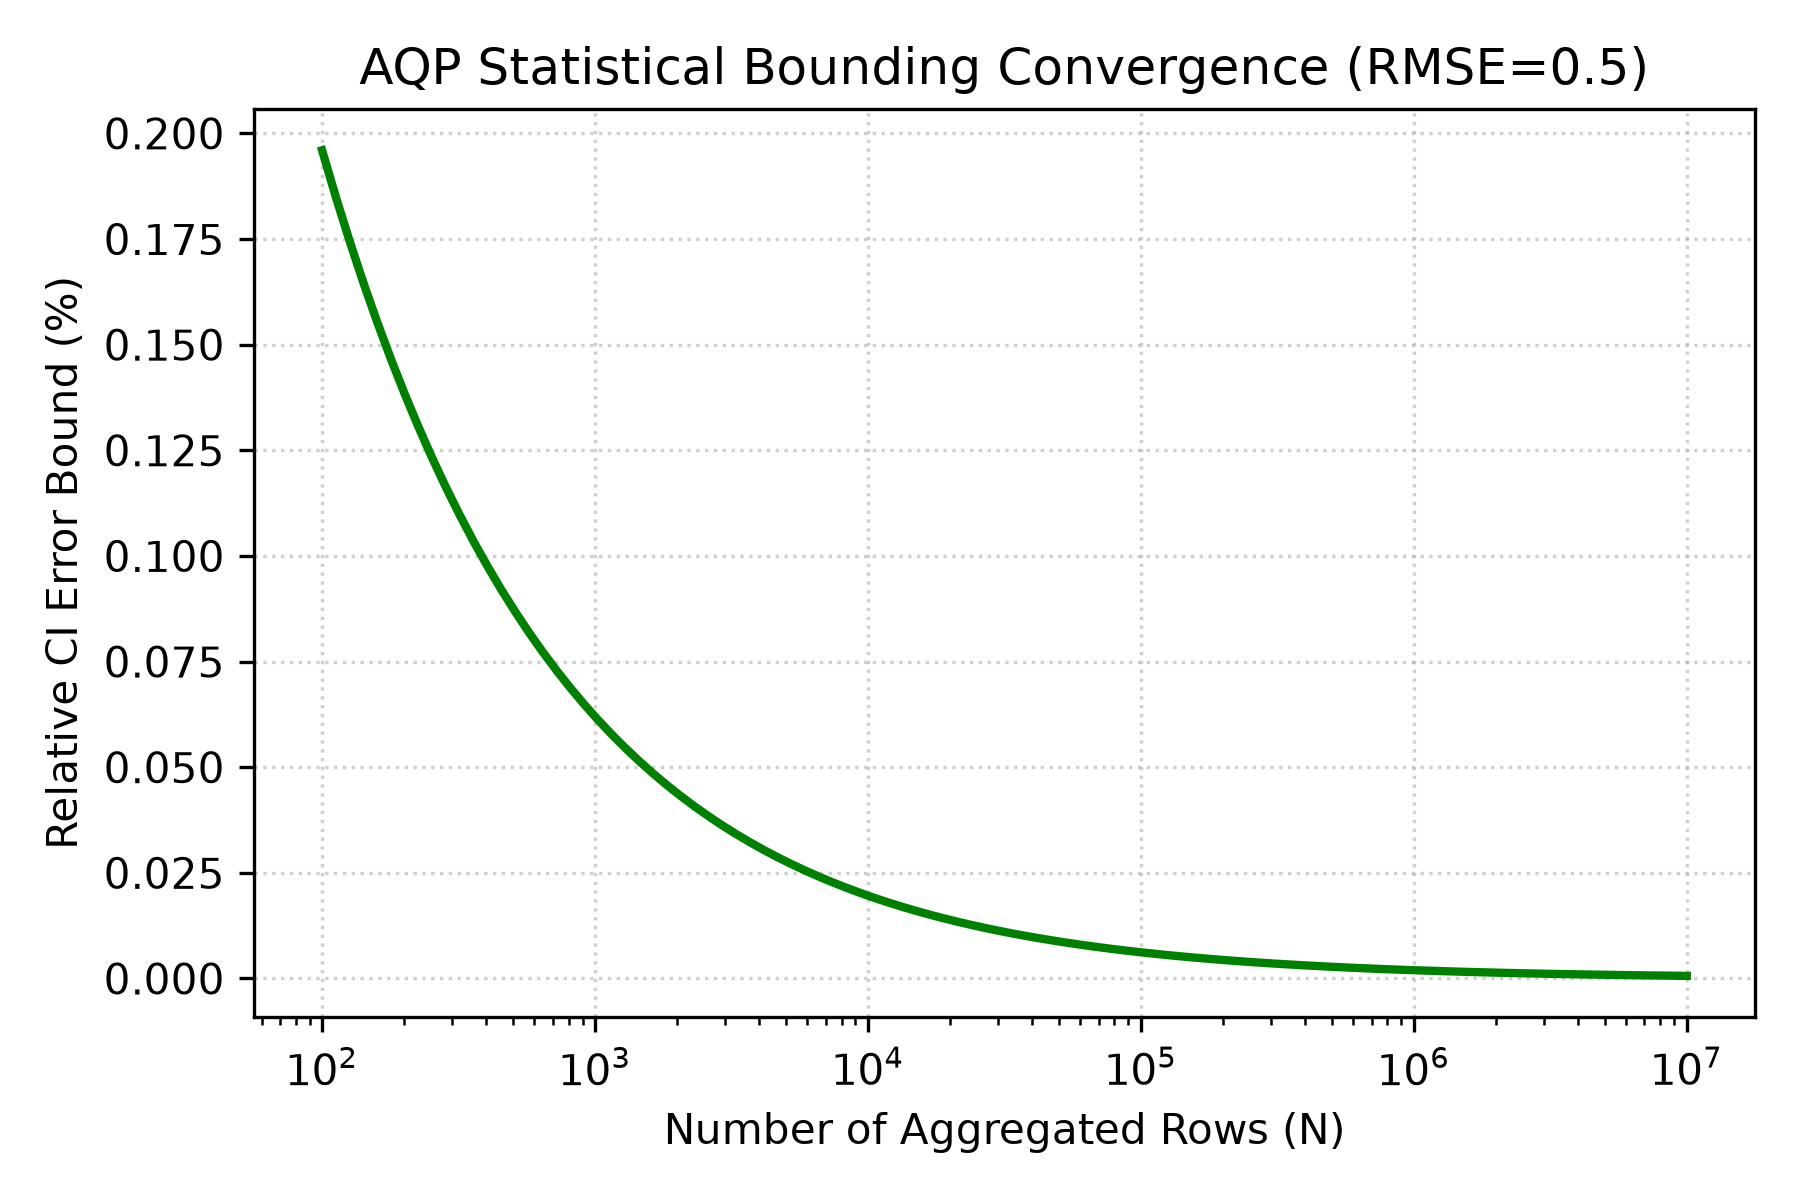
\includegraphics[width=0.9\columnwidth]{images/aqp_bench.png}
\caption{Theoretical AQP Convergence ($1/\sqrt{N}$). As the number of aggregated rows $N$ increases, the relative error bound logically shrinks, assuming strictly i.i.d unbiased errors.}
\label{fig:aqp}
\end{figure}

\section{Systems Evaluation}

We validate the architectural latency on an AMD Ryzen 9 5900X, 32GB RAM, 1TB NVMe SSD running Linux. Numbers represent the mean across 10 repeated trials. The ML model evaluates 2048 rows per batch across 12 threads. Note: Accuracy and empirical CI coverage of the predictions are completely out of scope.

\subsection{Stress Testing Selective Queries}
We generated 10,000,000 synthetic rows. We evaluate a highly selective query ($S = 0.05$) to demonstrate the systems benefits of lazy materialization vs a pre-computed Static Backfill.
\begin{verbatim}
SELECT category, sum_ci(val, rmse) 
FROM stress_data 
WHERE date >= '2023-11-01' -- 5% selectivity
GROUP BY category;
\end{verbatim}

\begin{table}[htbp]
\centering
\caption{End-to-End Latency Benchmark (10M Rows, $S=0.05$)}
\begin{tabular}{@{}lcc@{}}
\toprule
\textbf{Operation Phase} & \textbf{Deferred Columns} & \textbf{Static Backfill} \\
\midrule
\textit{Upfront Pipeline Cost} & & \\
Python Data Export & \textbf{0 ms} & 110.9 $\pm$ 26.2 ms \\
External ML Inference & \textbf{0 ms} & 584.6 $\pm$ 191.0 ms \\
Bulk UPDATE \& Commit & \textbf{0 ms} & 944.7 $\pm$ 250.0 ms \\
\midrule
\textit{Query Execution Cost} & & \\
Disk I/O \& Filter & 16.0 $\pm$ 2.0 ms & 16.0 $\pm$ 2.0 ms \\
ML Imputation (Lazy) & 364.2 $\pm$ 15.3 ms & 0 ms \\
Hash GroupBy \& AQP & 2.8 $\pm$ 0.2 ms & 2.8 $\pm$ 0.2 ms \\
\midrule
\textbf{Time-to-First-Insight} & \textbf{383.0 ms} & \textbf{1659.0 ms} \\
\bottomrule
\end{tabular}
\label{tab:results}
\end{table}

To ensure a fair baseline comparison, the external Static Backfill pipeline was aggressively optimized. Python data export utilized PyArrow zero-copy deserialization (\texttt{duckdb.fetch\_arrow\_table()}). External inference ran identical ONNX models via \texttt{onnxruntime} Python bindings. Finally, the commit phase utilized DuckDB's native \texttt{Appender} API to materialize the fully imputed dataset into a new table followed by an atomic swap, representing a best-case bulk materialization scenario.

As shown in Table \ref{tab:results}, Deferred Columns completely eliminates the 1.64-second upfront materialization pipeline inherent to external Python middleware. By parallelizing the inference within DuckDB's native multi-threaded table function pipeline, Deferred Columns achieves a Time-to-First-Insight of 383.0 ms, strictly outperforming Static Backfill's 1659.0 ms on the first query. However, because Deferred Columns intentionally avoids caching to maintain isolation, its execution latency remains 383.0 ms on every subsequent query, while Static Backfill drops to a mere 18.8 ms. 

This establishes a clear exploratory break-even point. Assuming identical ad-hoc analytical queries:
\begin{equation}
n \times 383.0 \leq 1640.2 + (n \times 18.8) \implies n \approx 4.5
\end{equation}
Deferred Columns is strictly superior for the first four exploratory queries. Once an analyst settles on a final query shape (query 5 and beyond), Static Backfill overtakes it. Thus, Deferred Columns serves as a high-speed lazy bridge for ad-hoc exploration, completely bypassing database locking and external state duplication.

\section{Limitations and Future Work}
Model accuracy and real-world CI coverage are out of scope for this systems evaluation and represent a crucial next step. Future iterations will dynamically calibrate $C_{inf}$ at runtime via sampling rather than static heuristics.

\section{Conclusion}
By building Deferred Columns natively in DuckDB, we have established a systems pipeline for lazy ML materialization. With MVCC-M isolation, cost-based pruning, and multi-threaded parallel execution, database engines can dramatically reduce the Time-to-First-Insight for exploratory analytics. Deferred Columns proves that skipping the expensive upfront backfill yields massive latency wins for initial data exploration, establishing a new paradigm for bridging machine learning and relational data.

\begin{thebibliography}{00}
\bibitem{imputedb} J. Cambronero, J. K. Feser, M. J. Smith, and S. Madden, ``Query Optimization for Dynamic Imputation,'' \textit{PVLDB}, 10(11), 2017.
\bibitem{quip} Y. Lin and S. Mehrotra, ``QUIP: Query-driven Missing Value Imputation,'' \textit{arXiv preprint}, 2022.
\bibitem{zip} Y. Lin and S. Mehrotra, ``ZIP: Lazy Imputation during Query Processing,'' \textit{VLDB Proceedings}, 2023.
\bibitem{tesseract} T. Hu, T. Wang, and Q. Zhou, ``Online Schema Evolution is (Almost) Free for Snapshot Databases,'' \textit{PVLDB}, 16(2), 2023.
\bibitem{mindsdb} MindsDB Inc., ``MindsDB: Machine Learning in the Database,'' \url{https://mindsdb.com}, 2019.
\bibitem{madlib} J. M. Hellerstein et al., ``The MADlib Analytics Library or MAD Skills, the SQL,'' \textit{PVLDB}, 5(12), 2012.
\bibitem{blinkdb} S. Agarwal et al., ``BlinkDB: Queries with Bounded Errors and Bounded Response Times,'' \textit{EuroSys}, 2013.
\bibitem{verdictdb} Y. Park et al., ``VerdictDB: Universalizing Approximate Query Processing,'' \textit{SIGMOD}, 2018.
\end{thebibliography}

\end{document}
